\chapter{Hierarchical Control for Team-Based Multi-Agent Racing}
% \epigraph{\flushright The Prestige}{}
\epigraph{\flushright But you wouldn't clap yet. Because making something disappear isn't enough; you have to bring it back. That's why every magic trick has a third act, the hardest part, the part we call ``The~ Prestige.''}{Christopher Priest, \textit{The Prestige}}
\label{chapter:team}
The final part of this report introduces another important facet of real-life racing into consideration: teamwork. Most professional racing series involve two competitions that run concurrently. There is an individual competition amongst the drivers, but there is also a competition over the performance of the racing teams based on the finishing positions of their respective drivers. Therefore, drivers are required to race with a mix of cooperative and competitive objectives in mind. We start by providing a motivating example of a team-based racing scenario where there exist several reasonable strategies, which may not be obvious to choose from. Next, we update the formulations discussed in the prior two chapters to generalize them to a team-based racing scenario. We conclude by evaluating our hierarchical control variants against the baselines introduced in the previous chapter in simulated races of four players with two on each team. This chapter is an extended discussion of work titled, ``Hierarchical Control for Cooperative Teams in Competitive Autonomous Racing'' co-authored with Aryaman Singh Samyal, David Fridovich-Keil, Zhe Xu, and Ufuk Topcu \cite{thakkarprior2}.

\section{Motivating Example}
\begin{figure}
  \centering
  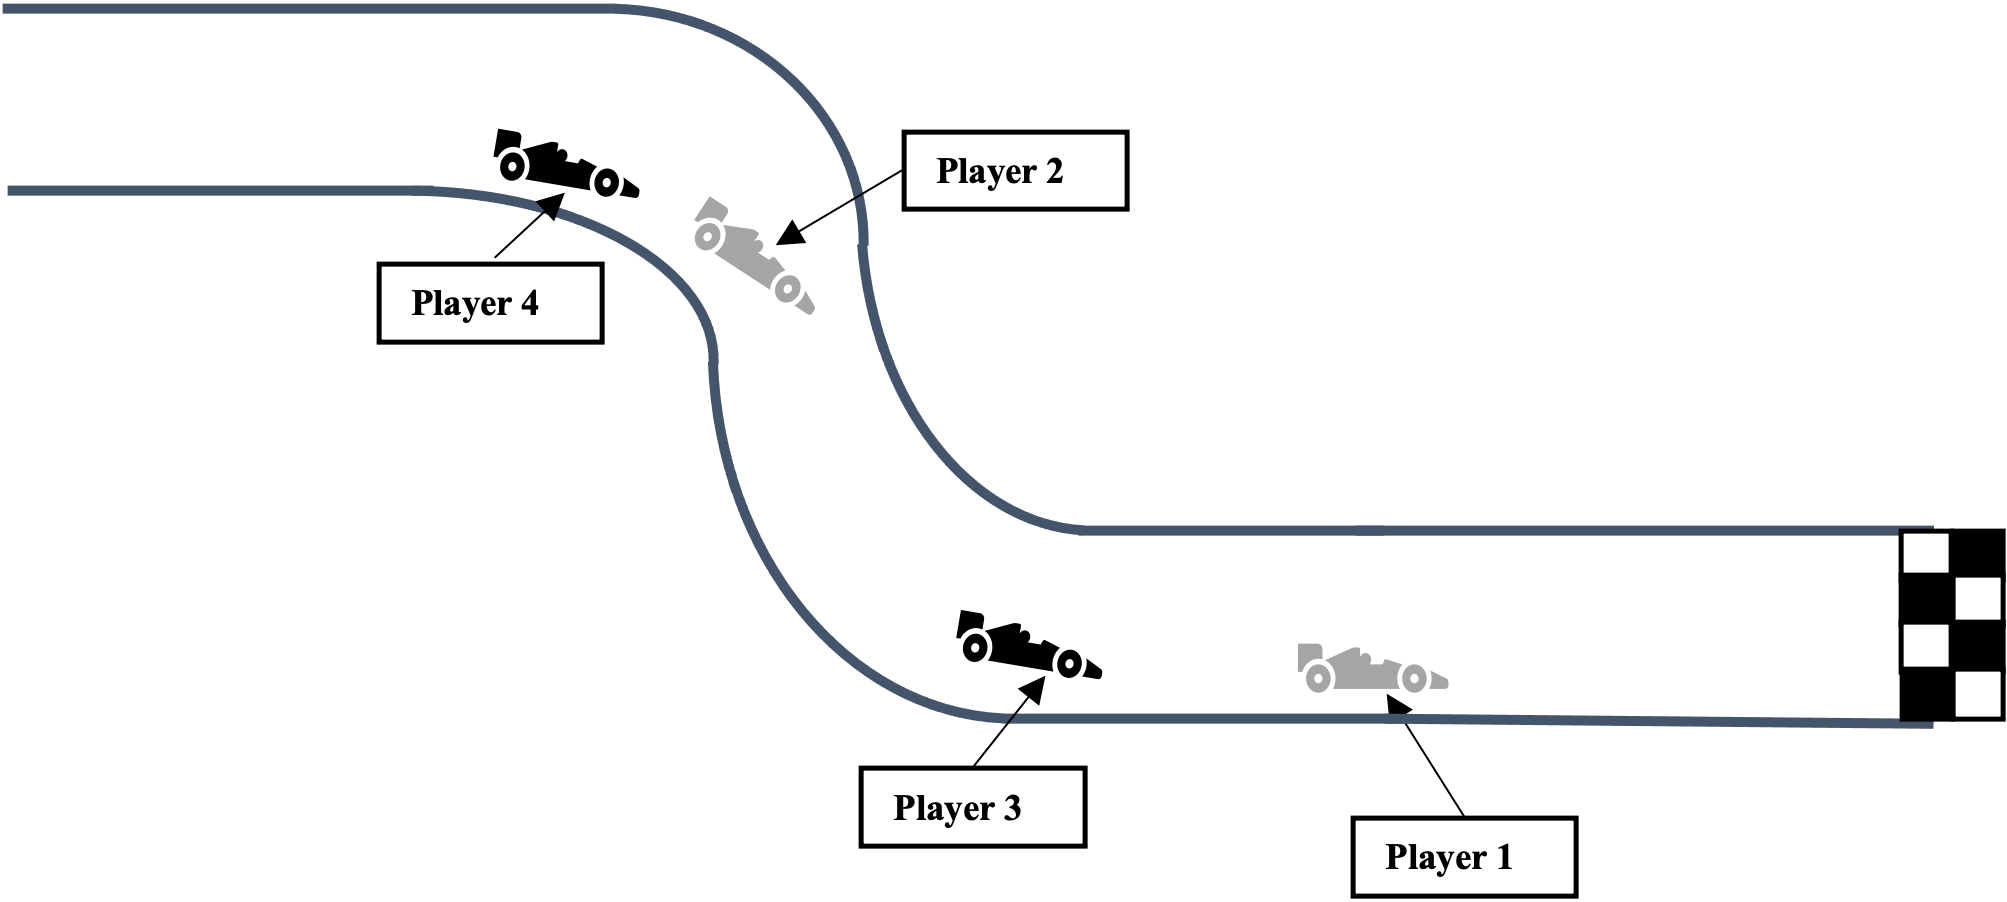
\includegraphics[width=\textwidth]{Figures/TeamMotiv.png}
  \caption[Motivating example for team-based racing] {Player 3's strategy is unclear. Should it try to pass Player 1, slow down on purpose to try help Player 4 pass Player 3, or maintain its position?}
  \label{fig:team_motivating}
\end{figure}

Consider the example in Figure \ref{fig:team_motivating}. Player 1 and Player 2 are on one team, and Player 3 and Player 4 are on another team. Player 1 is clearly first and almost at the finish line, so it is unlikely that Player 3, who is second, can catch it before the finish line. On the other hand, Player 4 is last, but he is close to Player 2 in third. Player 3 now has three high-level choices to consider:
\begin{enumerate}
    \item Try to overtake Player 1 before the finish line.
    \item Maintain its position to the finish line.
    \item Purposely slow down with the risk of being passed by Player 2 but also improve the chances of Player 4 overtaking Player 2 by slowing down Player 2.
\end{enumerate}
If all players were racing independently, choice 1  would likely be the most reasonable because that is only possibility of any payoff. However, because there is an incentive to finish higher overall as a team, Player 3 must consider the payoffs from all three choices. The payoffs and the risks associated with these choices are not necessarily obvious to evaluate. The implications of the choices are not immediately observed, and it is usually challenging to switch from one choice to the next. For example, committing to choice 3 means that Player 3 cannot realistically change its mind and switch to choice 1 if it realizes the risk is too high. 

We have discussed in prior chapters how the original formulation, before the introduction of team-based objectives, is already a challenging problem to tackle. Adding these complexities only makes the problem more difficult. Therefore, we propose that using our hierarchical control structure is even more vital in these scenarios as it allows players to evaluate the long-term implications of complex strategies while still adhering to the rules of the game. To study the impact of our method performs in these scenarios, we begin by generalizing all of our racing game formulations to the team-based setting.

\section{Formulation Updates for Team-based Racing}
To adapt each of our formulations for team-based racing, we introduce some additional notation to indicate how the teams are organized and describe how to update the objective function to reflect both competitive and cooperative goals. The constraints in the game remain the same as players still must follow the safety and fairness rules regarding lane changes, collision avoidance, and track constraints.
\subsection{General Racing Game Formulation}
We introduce a set $M$ consisting of mutually exclusive subsets of players in $N$. Each of the sets in $M$ represents a team of players who have a share the objective of also improving the teams overall finishing positions. We introduce a multiplier $\zeta \in [0,1]$ to balance a player's emphasis on its team objective vs. its personal objective. For a player $i$ on team $\mu$, the updated objective of the general formulation is as follows:
\begin{equation} \label{eq:gen_team_obj}
    \min_{u^i_0, ..., u^i_T} \gamma^i+\zeta (\sum_{j \in \mu \setminus i} \gamma^k) - \frac{(1+\zeta(|\mu|-1))\sum_{j \in N \setminus \mu }\gamma^j}{|N|-|\mu|} 
\end{equation}
If $\zeta=0$, then the objective closely resembles the head-to-head case but is different in that the player is only minimizing its pairwise differences in finishing time with all other players, not on its team. If $\zeta=1$, the player places equal emphasis on its own finishing time with that of all other members of its team. Lastly, this objective function does generalize to the head-to-head racing scenario studied previously because each player's team set would contain 1 just one element, i.e. $|\mu|=1$, and the value of $\zeta$ would be irrelevant. 

\subsection{High-Level Discrete Game Formulation}
The updated discrete game objective has a similar form to the updated objective of the general game formulation because both of have a similar structure in their original form. We reuse the same symbols introduced in the prior section and chapters. The updated reward function for player $i$ in the discrete game on team $\mu$ and a team performance multiplier is:
\begin{equation}
    R^i(s^1, ... s^n) = \begin{cases} 
                \frac{(1+\zeta(|\mu|-1))\sum_{j \in N \setminus \mu} s^j_t}{|N|-|\mu|} - s^i_t - \zeta(\sum_{j \in \mu \setminus i} s^k_t) & \text{if } (\bigwedge_{p \in N} s^p_k   = c_\tau) \\ 
                0    & \text{otherwise}
                \end{cases}
\end{equation}
 The players aim to maximize the difference between a scaled score of all other opponent's finishing times and their teammates' and own finishing times. Similar to the updated objective described in the previous section $\eta$ balances the cooperative and competitive objectives.
\subsection{Low-Level Simplified Game Formulation}
Even though we do not directly solve the low-level formulation introduced in the previous chapter, we provide an updated objective function here for completeness. In the original low-level formulation, the objective is to maximize the checkpoint difference at the end of the planning horizon. We use the similar trick of multiplying the performance of teammates by a factor $\zeta$ and normalizing the scores based on the number of opponents and teammates. The updated objective for player $i$ on team $\mu$ playing the low-level game is:
\begin{equation} \label{eq:ll_team_obj}
    \min_{u^i_{1}, ..., u^i_{\delta}} (\frac{((1+\zeta(|m|-1))\sum^N_{j \in N\setminus \mu}r^j_{\delta}}{|N|-|m|} -  r^i_{\delta} - \zeta\sum_{j \in \mu \setminus i}r^j_\delta) \; +  
    \alpha \sum_{c={r^i_{1}}}^{{r^i_{1}}+k} \eta^i_c
\end{equation}

Again, there are two parts to the low-level objective. The first part incentivizes players to pass as many checkpoints as possible as a team. The second part incentivizes the individual player to hit its target waypoints as closely as possible. The second part remains unchanged from the original formulation, but the first part considers the team's overall count of passing the checkpoints within the fixed time horizon. 

We do not directly solve the low-level simplified formulation, but rather integrate into a MARL-based model and further simplify it into an LQNG representation. Therefore, in the following subsections, we discuss how the implementation of these controllers is updated to represent the updated objective of the low-level game.

\subsubsection{Multi-Agent Reinforcement Learning Controller}
We make two changes to our MARL model to reflect the changes in the updated low-level formulation. First, we update the reward structure to incorporate the overall team-performance calculations. We introduce a shared reward for all agents of a team using the order in which the checkpoints are passed resembling the points that are awarded to teams based on their driver's finishing positions in real-life racing. Using this shared reward mechanism connects to the second change to the MARL model, which is changing the learning algorithm used to train the control policy. We use an algorithm called posthumous counterfactual credit assignment) developed by the creators of Unity ML-Agents library \cite{poca}. Their algorithm is an extension of the state-of-the-art counterfactual multi-agent policy gradients algorithm developed by \citet{coma}. In their extension, the scientists at Unity modify how team rewards impact the policy after an agent might have reached the end of its life while the other players in the system may still be active. In our case, the end of an agent's life refers to finishing the race. 

\subsubsection{Linear-Quadratic Nash Game Controller}
Updating the LQNG-based controller does not require any explicit changes to the LQNG formulation. In the original LQNG formulation, we introduced a series of multipliers $\rho$ that is multiplied by other players' distances to their upcoming waypoints in the second component of the objective \eqref{eq:lqng_obj2}. We ensure the signs of those multipliers for the players on the ego player's team are negative. By doing so, the player will no longer have an objective to hinder those players' progress towards their checkpoints; instead, it will be rewarded for selecting trajectories that aid its teammates in reaching their target waypoints. 

\section{Team-based Racing Results}
Our experiments include 2v2 team racing on a basic oval track (which the learning-based agents were trained on) and a more complex track (which they were not trained on) shown in Figure \ref{fig:experiment_tracks}. Each team is composed of two players both using one of the five types of implemented controllers, MCTS-RL, MCTS-LQNG, E2E, Fixed-LQNG, and Fixed-RL, constructing five teams. Every pair of teams competes head-to-head in 48 races on both tracks. The dynamical parameters (cornering limitations, top speed, acceleration, braking, etc.) of each player's vehicle are identical. The only difference in their initial states is the lane in which they start and the initial checkpoint. Two of the players start \SI{10}{\meter} in front of the other pair resembling the starting grid of real-life racing. To maintain fairness with respect to starting closer to the optimal racing line or ahead of others, we rotate through each of the six unique ways to place players at the four possible starting positions.

Our experiments seek to reinforce the importance of hierarchical game-theoretic reasoning and study its scalability to challenging problems with strategies requiring coordination in addition to competition when long-term planning. We are also interested in observing maneuvers where teammates use tactical positioning to help pass or defend against the opposing team, commonly seen in expert human racing. We assign points to each of the four finishing positions, $[10, 7.5, 6, 4]$ and $0$ for not finishing the race. The points are summed at the end of the race for each team. The number of points is important because it measures the overall performance of the team rather than the individual ability of a specific controller. Nevertheless, for each team, we still count the number of wins (i.e. 1st place finishes), average collisions-at-fault per race, average illegal lane changes per race, and a safety score (a sum of the prior two metrics) to obtain a holistic view of the implemented controllers. Our analysis focuses on three key metrics: average points per race, wins, and safety score. Appendix \ref{app:team_results} provides tables with a complete breakdown of the results for every pair of teams. We also provide a video\footnote{\vidurlteam} demonstrating them in action. 

\begin{figure}
  \centering
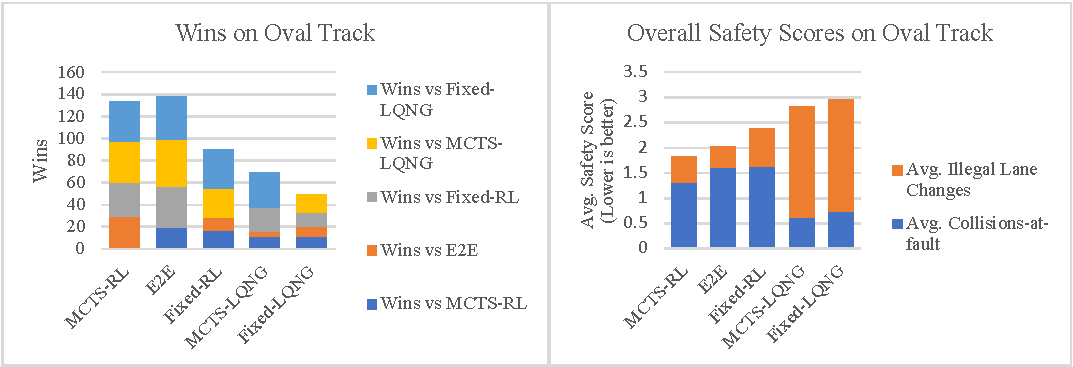
\includegraphics[width=\textwidth]{Figures/TeamOvalResultsFinal.pdf}
  \caption{Results from head-to-head racing on the oval track.}
  \label{fig:team_results_oval}
\end{figure}
\begin{figure}
\centering
  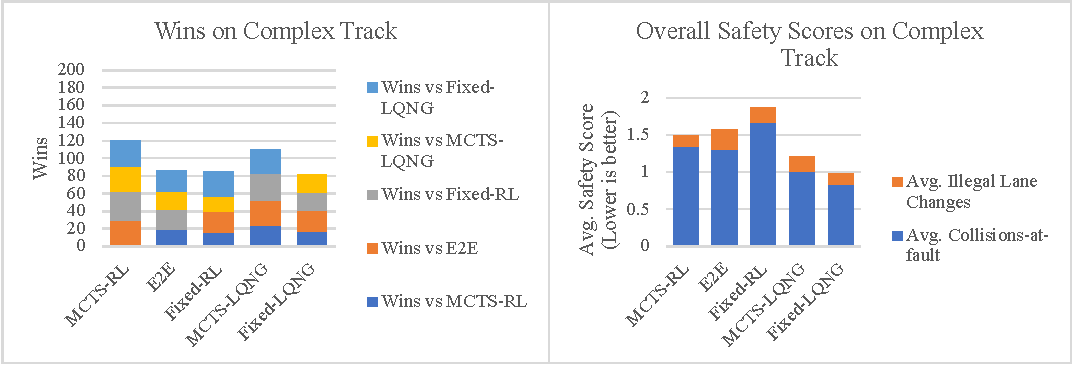
\includegraphics[width=\textwidth]{Figures/TeamComplexResultsFinal.pdf}
  \caption{Results from head-to-head racing on the complex track.}
  \label{fig:team_results_complex}
\end{figure}

\begin{table}[!ht]
    \centering
    \begin{tabular}{|p{4cm}|l|p{3.25cm}|p{3cm}|}
    \hline
        \textbf{Aggregate Results (384 Total Races)} & \textbf{Wins} & \textbf{Average Points Per Race} & \textbf{Average Safety Score} \\ \hline
        MCTS-RL & 254 & 14.93 & 1.61  \\ \hline
        E2E & 224 & 13.20 & 1.67  \\ \hline
        Fixed-RL & 175 & 13.51 & 2.14  \\ \hline
        MCTS-LQR & 175 & 12.89 & 1.91  \\ \hline
        Fixed-LQR & 132 & 12.56 & 1.78 \\ \hline
    \end{tabular}
    \caption[Aggregated team-based racing results.]{Aggregated team-based racing results across both tracks.}
    \label{tab:team_aggr_results}
\end{table}

Based on the plots in Figure \ref{fig:team_results_oval} and Figure \ref{fig:team_results_complex} and Table \ref{tab:team_aggr_results}, we conclude the following key points:

\begin{enumerate}[wide, labelindent=0pt, font=\bfseries]
% MCTS-based variants outperformed respective baselines
\item \textbf{The proposed hierarchical controllers scale to the challenge of team-based racing by continuing to outperform their respective baselines.} 

The results amongst MCTS-RL, Fixed-RL, and E2E continue to show the effectiveness of our hierarchical structure. Again, all of the MARL-based agents were trained only on the oval track, but MCTS-RL continues to lead in all of the key metrics. While MCTS-RL has more wins overall, the difference in the number of wins is not as high as in the head-to-head case. However, the essential metric of interest in this study is average points per race, which evaluates team-based performance. MCTS-RL maintains a considerable difference in terms of average points per race compared to the baselines. The higher points per race imply that even if MCTS-RL is not able to finish 1st, it collaborates more effectively to produce better results as a team. 

Next, comparing just the baselines, we notice that Fixed-RL is worse in terms of wins and safety score compared to E2E. Recall that the Fixed-RL controller simply follows a fixed optimal racing line. While such a strategy might be successful in the head-to-head case where there is only one opponent to consider, in the team racing scenario, it is imperative for players to consider alternative racing lines especially if one's teammate is already following a specific line. As a result, Fixed-RL often had collisions with its own teammate as both players competed over the same space. In those situations, one or both of the Fixed-RL teammates sometimes lost a position. However, once they were separated far enough after recovering from the collision, the agents on the Fixed-RL team could both drive fast enough to at least maintain their new positions or independently overtake their opponents, which is reflected in its higher points-per-race score compared to E2E. This pattern implies that hierarchical reasoning is important to be quick, but is not necessarily enough. To be the most successful, game-theoretic hierarchical reasoning, e.g. MCTS, should be used to allow teammates to predict each other's plans and work together effectively. 

Finally,, we compare MCTS-LQNG and Fixed-LQNG. Both LQNG agents have similar safety scores. However, MCTS-LQNG still has 33\% more wins and a better points-per-race metric overall. Again like the head-to-head case, the main drawback with the fixed trajectory tracking agents is that they do not consider alternative racing lines. While in the head-to-head case considering alternative lines might not be as important, it becomes considerably more vital to success in multi-agent multi-team racing.

% RL is better than LQNG for low-level
\item \textbf{MARL continues to perform better than LQNG as a low-level planner but, the difference in the metrics is smaller in team-based racing compared to head-to-head racing.}  

Across both tracks, the MARL-based agents are still generally better than the LQNG-based agents in terms of our key metrics. However, the difference in their performance is narrowed compared to the head-to-head case. For example, in the complex track, both the LQNG-based agents have better safety scores than their MARL-based counterparts, but in the oval track, the scores are significantly worse due to the number of illegal lane changes by the LQNG-based agents. As discussed in the analysis of the head-to-head racing results in Chapter \ref{chapter:hier}, the LQNG-based controllers are conservatively tuned for collision avoidance due to their short horizons. Therefore, they continue to maintain fewer collisions-at-fault, but this setup also forces them to change lanes more often to avoid collisions, especially given that there are more players in the game. Furthermore, it also results in the LQNG-based agents often conceding in close battles and thereby losing races because of the high cost in the planning objective of driving near another player even if there is no collision. Despite that, MCTS-RL has just 45\% more wins in the team-based experiments compared to the 80\% more wins it has against MCTS-LQNG in the head-to-head experiments. For the fixed trajectory agents, this gap drops from 250\% to 33\%. Nevertheless, when we consider our primary metric evaluating team-based performance, points-per-race, both MARL-based variants are better than the LQNG-based variants, but the gap between Fixed-RL and Fixed-LQNG is smaller than the gap between MCTS-RL and MCTS-LQNG. Overall, all of the metrics are still in favor of using the MARL-based agents because they are generally more robust to nuances of the many possibilities of situations that arise. On the other hand, our LQNG formulation has a mixture of concave and convex components in the objective function, is only linearized around the initial state, and uses short horizons, so our cost surface is sometimes unreliable degrading the resulting behavior as also discussed in the results of the head-to-head experiments.

% MCTS-RL is the best overall controller.
\item \textbf{MCTS-RL outperforms all other implemented controllers exhibiting teamwork tactics resembling real-life experts.}  

The MCTS-RL team records a win rate of over 66\% of the 384 races it participated in across both tracks, the best overall safety score, and the highest points per race. The MCTS high-level planners provided the agents with a series of waypoints allowing them to make decisions in complex tactical situations where there is a mix of both competitive and cooperative objectives. The MARL-based low-level planner provided robustness to adapt to the true scenario that plays out. Although the players do not communicate or explicitly coordinate strategies, they still produce cooperative behaviors that improve their overall performance as a team. 

We also observe our controllers execute plans that resemble those performed by expert human drivers. For example, Figure~ \ref{fig:team_mctsrl:overtake} demonstrates how the two high-level planners of each MCTS-RL agent developed a strategy to perform a pincer-like maneuver to overtake an opponent. Both agents from the MCTS-RL team approached the opponent from either side of the opponent at the same time. The opponent could only defend one of the agents on the MCTS-RL team allowing the other agent on the team to pass. In addition, MCTS-RL is also successful at executing strategic maneuvers as seen in Figure~ \ref{fig:team_mctsrl:strategy} where an agent, who is ahead, momentarily slows down and blocks an opponent behind to allow for its teammate to pass the opponent. Both of these tactics resemble strategies of expert human drivers in real head-to-head racing.
 \end{enumerate}
 
 \begin{sidewaysfigure}
  \centering
  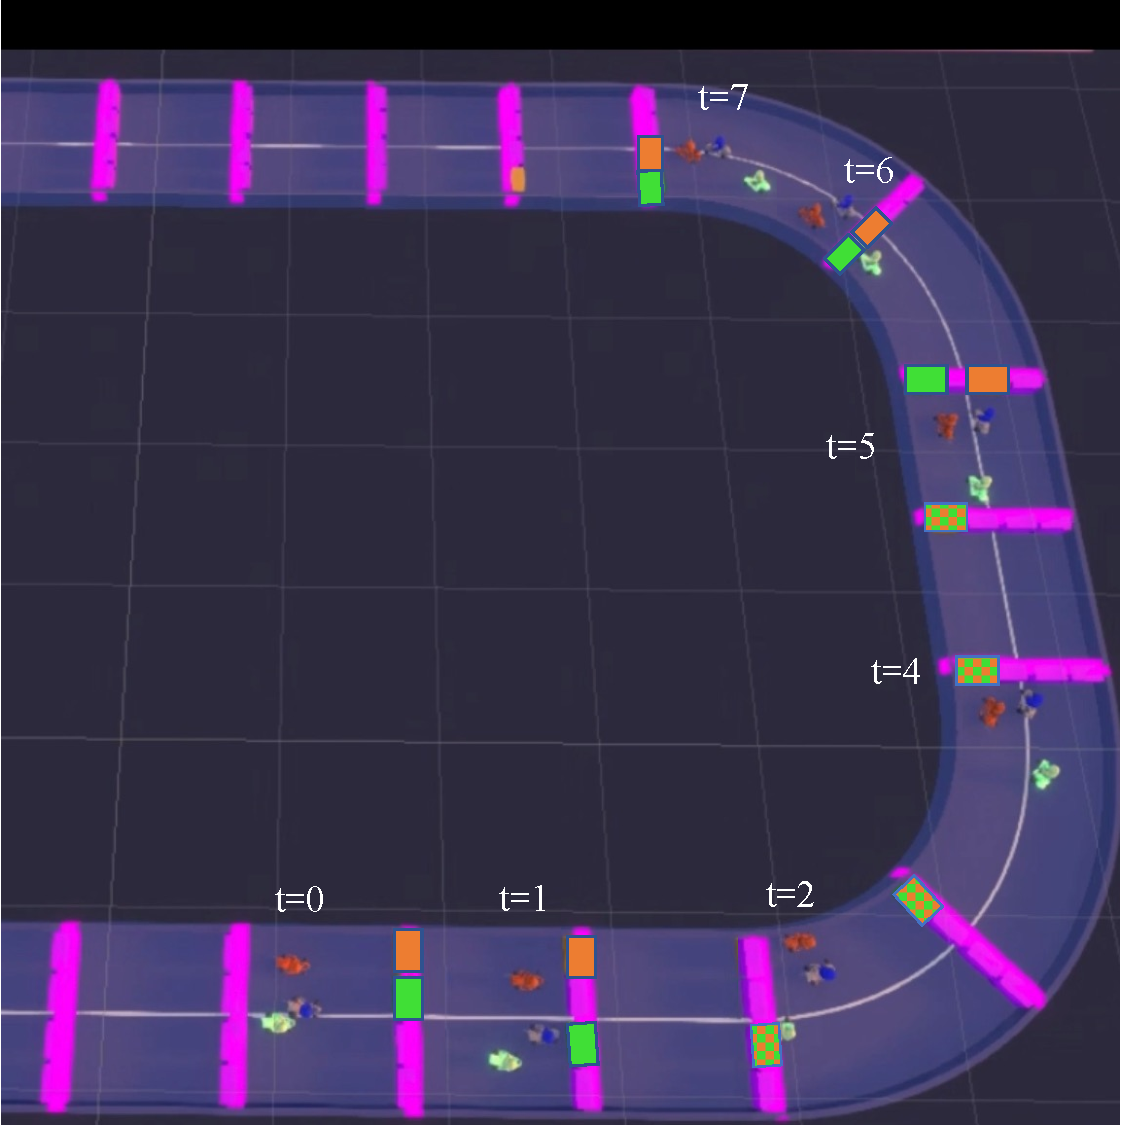
\includegraphics[height=0.7\textheight]{Figures/MCTSRLTeamOvertake.pdf}
  \caption [Overtaking maneuver by team of MCTS-RL agents.] {An overtaking maneuver executed a team MCTS-RL agents (green and orange) against the Fixed-RL agent (blue) on the oval track. From $t=0$ to $t=1$, the MCTS-RL agents split and attack the Fixed-RL agent from both sides. The Fixed-RL agent attempts to defend the green MCTS-RL agent on its right allowing the orange MCTS-RL agent to overtake on its left from $t=2$ to $t=6$. The green and orange boxes along each checkpoint highlight the long-term plans calculated by the MCTS planners of each of the MCTS-RL agents, respectively. The checkered boxes indicate a shared checkpoint in their plans.}
  \label{fig:team_mctsrl:overtake}
\end{sidewaysfigure}

\begin{sidewaysfigure}
 \centering
  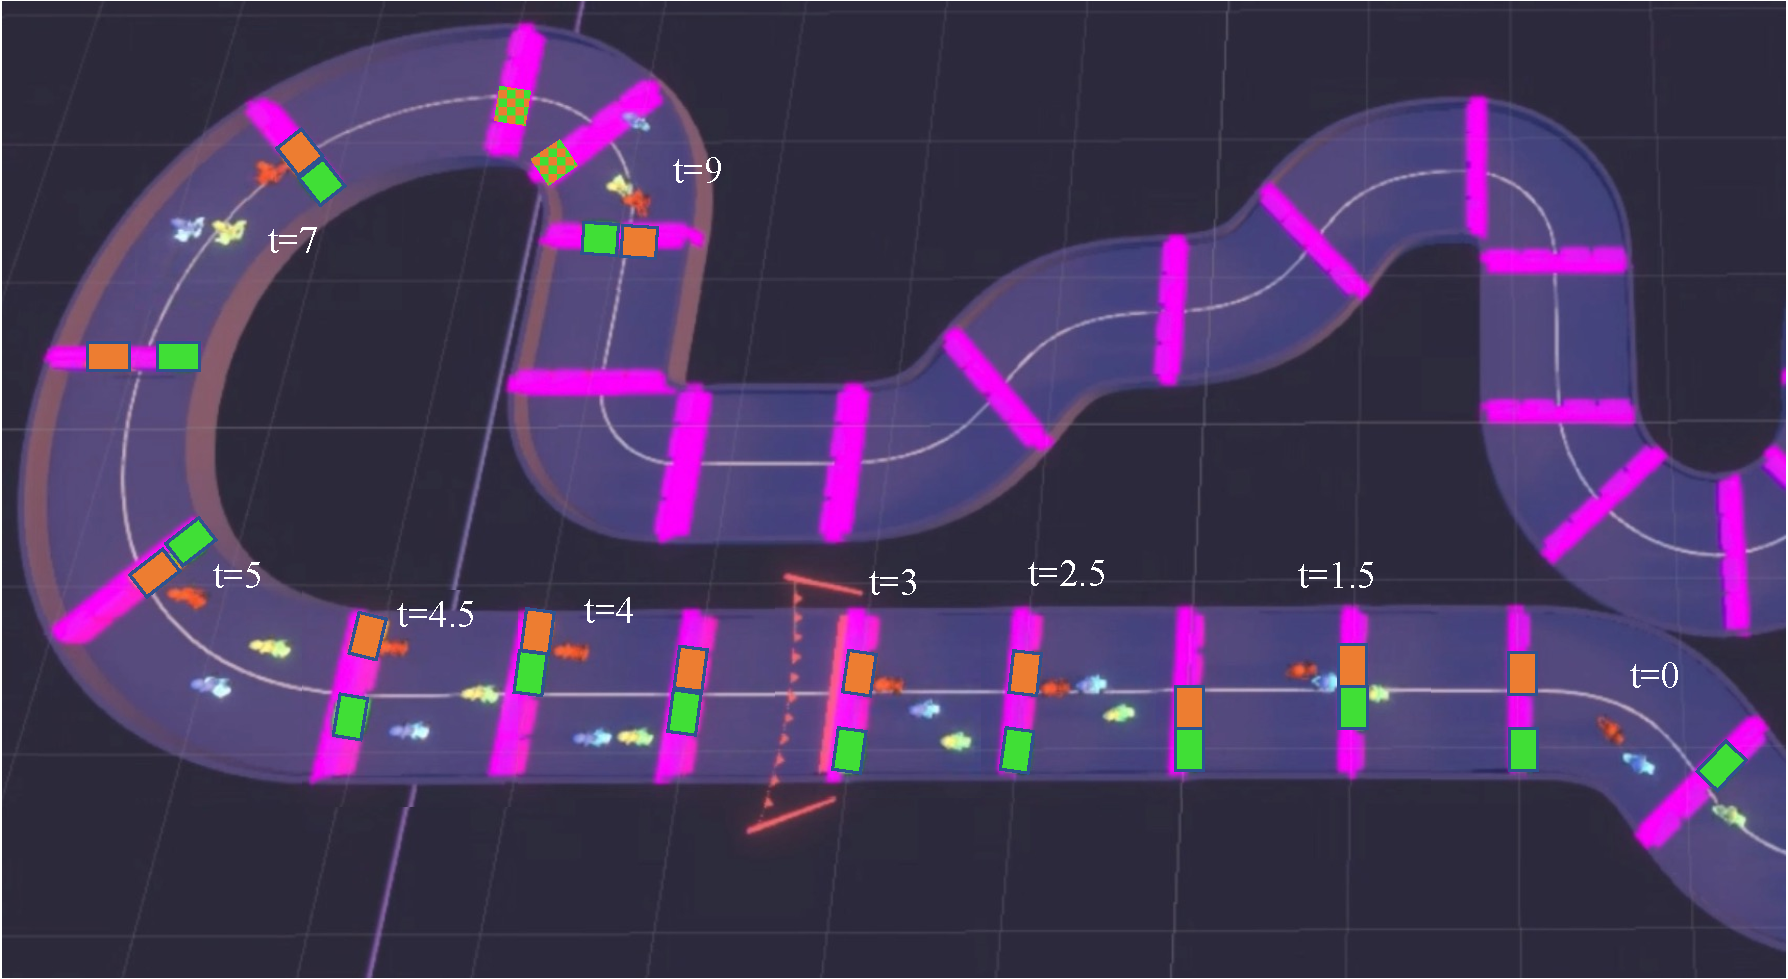
\includegraphics[width=\textwidth]{Figures/MCTSRLTeamBlockToOvertake.pdf}
  \caption[Block to overtake maneuver executed by the team of MCTS-RL agents.]{A tactical maneuver executed by the MCTS-RL team (green and orange) against an E2E agent (blue) on the complex track.  Before reaching the turn, the green MCTS-RL's high-level planner calculates a trajectory suggesting to switch lanes to the left for the first part of the upcoming straight and to block the E2E agent forcing it to slow down and evade further to the left of the track ($t=0$ to $t=3$). This blocking move allows the orange MCTS-RL to plan to take advantage of the opponent's disruption and quickly switch to the right for the inside line of the upcoming turn ( $t=3$ to $t=5$). Eventually, the orange MCTS-RL agent completes the overtake by $t=9$. The green and orange boxes along each checkpoint highlight the long-term plan calculated by MCTS planners of each of the MCTS-RL agents, respectively. The checkered boxes indicate a shared checkpoint in their plans.}
  \label{fig:team_mctsrl:strategy}
\end{sidewaysfigure}
